\subsection{Observed TCEs}

\label{s:tces}
As with the previous three Kepler planet candidate catalogs \citep{Coughlin2016,Mullally2015cat,Rowe2015cat}, the population of events that were used to create KOIs and planet candidates are known as \opstce s. These are periodic reductions of flux in the light curve that were found by the Transit Planet Search (TPS) module and evaluated by the Data Validation (DV) module of the Kepler Pipeline \citep{JenkinsKDPH}.   The Data Release 25 \opstce s were created by running the SOC 9.3 version of the \Kepler\ Pipeline on the DR25, Q1--Q17 \Kepler\ PDC time-series.  For a thorough analysis of the DR25 TCEs and on the pipeline's search see \citet{Twicken2016}. 

The DR25 \opstce s, their ephemerides, and the metrics calculated by the pipeline are available at the NASA Exoplanet Archive \citep{Akeson2013}.  In this paper we endeavor to disposition these signals into planet candidates and false positives.  Because the \opstce s act as the input to our catalog, we first describe some of their properties as a whole and reflect on how they are different than the previous \Kepler\ TCE tables.

We have plotted the distribution of the \ntcesnorogue\ \opstce s in terms of period in Figure~\ref{f:obstces}. Notice, an excessive number of short and long period \opstce{s}. Also the number of \opstce{s} increeases with decreasing MES. 

As with previous catalogs, the short period ($<10$\,d) excess is dominated by true, sinusoidal variability of the star. The long period excess is dominated by instrumental noise. For example, a decrease in flux following a cosmic ray hit (a.k.a. SPSD, Sudden Pixel Sensitivity Drop-out \citep{KDCH}), can match-up with stellar variability to produce a TCE. Also, image artifacts known as rolling-band is very strong on some channels \citep[see \S6.7 of][]{KIH}  and since the spacecraft rolls every $\approx$90\,days, causing a star to move on/off a \Kepler\ detector with significant rolling band, these variations can easily line-up to produce TCEs at 372\,d. This is the reason for the spike in the \opstce\ population seen in Figure~\ref{f:obstces}. Generally, the excess of long period TCEs is significantly larger than it was in the DR24 TCE catalog \citep{Seader2015}. Most likely, this is because DR24 implemented an aggressive and irregular veto known as the bootstrap metric \citep{JenkinsBootstrap}.  For DR25 this metric was calculated, but was not used as a veto. Also other vetoes were made less strict causing more TCEs across all periods to be created. 

To summarize, for DR25 the number of false signals among the \opstce s  is dramatically larger than in any previous catalog. As a result, we expect the \opstce\ list to contain more true exoplanets than before.   

\begin{figure}[h!]
 \begin{center}
  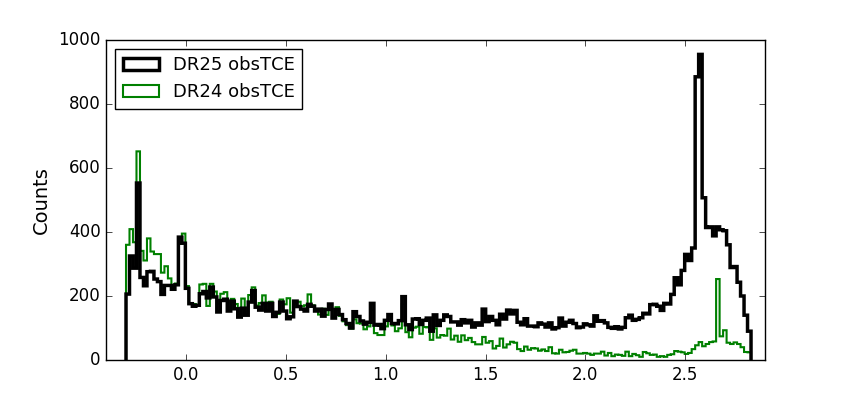
\includegraphics[width=1.0\linewidth]{fig-obstcePeriods.png}
  \caption{Histogram of the log$_{10}$(period) in days of the \opstce{s} (black). The DR24 catalog obsTCEs \citep{Seader2015} are shown in green for comparison. The number of long period TCEs is much larger for DR25, requiring a more effective Robovetter than in DR24.}
  %\caption{\ref{f:tces} A two dimensional histogram of the number of TCEs by log(period) and log(MES). The marginalized distributions for log(period) and log(MES) are projected along their respective axes and shown on the top and right respectively. }
  \label{f:obstces} 
 \end{center}
 \end{figure}



\subsection{Rogue TCEs}
The DR25 TCE table at NExScI contains \ntcesnorogue\ \opstce{s} and 1498 rogue TCEs for a total of \ntces. The rogue TCEs were created because of a bug in the Kepler pipeline which let through certain three-transit events. Because the primary purpose of this catalog is to be able to accurately calculate occurrence rates and because this same bug was not present when characterizing the completeness of the \Kepler\ Pipeline \citep{Christiansen2017,Burke2017a,Burke2017b,Burke2017c}, we ignore the rogue TCEs here. Also note that all of the TCE populations (observed, injection, inversion and scrambling, see the next section) had rogue TCEs. The creation and analysis of this KOI catalog only rely on the non-rogue TCEs.

